\documentclass[t]{beamer}

\mode<presentation> {\usetheme{Madrid}}

\usepackage{graphicx} 
\usepackage{booktabs}
\usepackage{braket}
\usepackage{amsmath}
\usepackage{mathtools}
\usepackage{verbatim}
\usepackage[makeroom]{cancel}


%----------------------------------------------------------------------------------------
%	TITLE PAGE
%----------------------------------------------------------------------------------------

\title[Gravitational Solitons from Topology]{Gravitational Solitons from Topology}

\author[Tasos Bouzikas]{Tasos Bouzikas\\{\scriptsize Supervised by: Bert Vercnocke (UvA)}}
\institute[UU] {Utrecht University}
\date{\today}

\titlegraphic{
\includegraphics[width=4cm]{uu-logo}}

\begin{document}

\begin{frame}
\titlepage
\end{frame}

%----------------------------------------------------------------------------------------
%	MAIN
%----------------------------------------------------------------------------------------

\begin{frame}
\frametitle{Introduction - Black Holes}

\begin{itemize}
\setlength{\parskip}{15pt}
\item<1-> Black Holes are solution to the Einstein Field Equations

\item<2-> Black Holes in General Relativity $(d = 4)$

\begin{itemize}
\setbeamertemplate{itemize items}[triangle]
\setlength{\parskip}{5pt}
\item Schwarzschild Black Hole ($M$)
\item Reissner - Nordstrom Black Hole ($Q$)
\item Kerr Black Hole ($J$)
\setbeamertemplate{itemize items}[default]
\end{itemize}


\item<3-> No-Hair Theorem: ``All black hole solutions can be completely characterised by only three parameters: $M$, $Q$, $J$.''

\item<4-> Add extra dimensions $\rightarrow$ Superstring Theory $(d=10)$ \:\:\: (LATER!!!)
\end{itemize}
\end{frame}

%------------------------------------------------ 

\begin{frame}
\frametitle{Introduction - Conserved Charges}

\begin{itemize}
\setlength{\parskip}{17pt}

\item<1-> Way to define these 3 quantities: $M,Q,J$ (conserved charges)

\item<2-> Motivated by the easiest one: $Q_{\text{\:Electric Charge}}$

\item<3-> Electrodynamics

\begin{itemize}
\setbeamertemplate{itemize items}[triangle]
\setlength{\parskip}{5pt}
\item Bianchi Identity: $dF = 0$
\item<4-> Equations of Motion: $d*F = *j$ \:\:\: $\rightarrow$ \:\:\: $d*j = 0$ (Conserved Current)
\item<5-> Conserved Charge:
\begin{align}
Q = \int\limits_{\Sigma} *j = \int\limits_{\Sigma} d*F = \int\limits_{\partial\Sigma} *F = Q_{\text{\: Electric Charge}} \notag
\end{align}

\setbeamertemplate{itemize items}[default]
\end{itemize}

\end{itemize}
\end{frame}

%------------------------------------------------ 

\begin{frame}
\frametitle{Introduction - Conserved Charges}

\begin{itemize}
\setlength{\parskip}{10pt}
\item General Relativity

\begin{itemize}
\setbeamertemplate{itemize items}[triangle]
\setlength{\parskip}{10pt}

\item<1-> We would like to have a similar expression for $M$ and $J$
\item<2-> (We are not going to deal with $J$ in this project!) 
\item<3-> Define $j^\mu = R^{\mu\nu} K_\nu $ $\rightarrow$ \:\:\: $\nabla_\mu j^\mu = 0$ (Conserved Current)
\item<4-> Conserved Charge:
\begin{align}
Q = \int\limits_{\Sigma} *j = \int\limits_{\Sigma} d*dK = \int\limits_{\partial\Sigma} *dK \notag
\end{align}
\setbeamertemplate{itemize items}[default]
\end{itemize}

\item<5-> Komar Integral
\begin{align}
\boxed{Q_{K} = \kappa_{d} \int\limits_{\partial\Sigma} *dK} \notag
\end{align}

\end{itemize}
\end{frame}

%------------------------------------------------ 

\begin{frame}
\frametitle{Introduction - Conserved Charges}

\begin{itemize}
\setlength{\parskip}{10pt}
\item<1-> Simplest Example: The Schwarzschild Black Hole

\begin{itemize}
\setbeamertemplate{itemize items}[triangle]
\setlength{\parskip}{5pt}
\item<2-> Schwarzschild Metric
\item<2-> Killing vector $K^\mu = (1,0,0,0)$

\vspace{0.1em}

\item<3-> By calculating $*dK$ and by choosing $\kappa_{d} = \frac{1}{8\pi G_4}$, we end up having:
\setbeamertemplate{itemize items}[default]
\end{itemize}

\item<4-> Komar Integral
\begin{align}
\boxed{
M = \frac{1}{8\pi G_4} \int\limits_{\partial\Sigma} *dK} \notag
\end{align}

\item<5-> Remember:  $j_\mu = R_{\mu\nu} K^\nu \xrightarrow[\text{Equation}]{\text{Einstein}} T_{\mu\nu} K^\nu \xrightarrow[\text{Component}]{\text{Temporal}} T_{00} \rightarrow M $

\end{itemize}
\end{frame}

%------------------------------------------------ 

\begin{frame}
\frametitle{Overview}

\begin{itemize}
\setlength{\parskip}{10pt}
\item<1-> Include Cosmological Constant $\Lambda$ (AdS Spacetime)
\item<2-> Include Topology
\item<3-> Include Matter Fields (Non - Empty Spacetime)
\item<4-> Interpret the result. Why 4 dimensions are not enough!
\item<5-> Moving to String Theory
\end{itemize}
\end{frame}

%------------------------------------------------ 

\begin{frame}
\frametitle{Overview}

\begin{itemize}
\setlength{\parskip}{10pt}
\item \boxed{\text{Include Cosmological Constant $\Lambda$ (AdS Spacetime)}}
\item Include Topology
\item Include Matter Fields (Non - Empty Spacetime)
\item Interpret the result. Why 4 dimensions are not enough!
\item Moving to String Theory
\end{itemize}
\end{frame}


%------------------------------------------------ 

\begin{frame}
\frametitle{Cosmological Constant $\Lambda$}

\begin{itemize}
\setlength{\parskip}{10pt}
\item<1-> Hilbert - Einstein Action
\begin{align}
S_{HE} = \frac{1}{2\kappa} \int d^dx \sqrt{-g} \Big( R - 2\Lambda \Big) \notag
\end{align}

\item<2-> Einstein Equations: $R_{\mu\nu} = \frac{2\Lambda}{d-2} g_{\mu\nu}$

\item<3-> Solution: AdS Spacetime 
\begin{align}
ds^2 = - \frac{r^2}{R^2} dt^2 + \frac{R^2}{r^2} dr^2 + r^2 d\Omega^2_2, \qquad \frac{1}{R^2} = \frac{2\Lambda}{(d-1)(d-2)}  \notag
\end{align}

\item<4-> The Komar integral diverges:
\begin{align}
Q_{K} = \int\limits_{\partial\Sigma}*dK = \int\limits_{\partial\Sigma} d\Sigma_{\mu\nu} \nabla^\mu K^\nu = \int\limits_{\partial\Sigma} d\Sigma_{tr} \frac{r}{R^2} \rightarrow \infty  \notag
\end{align}

\end{itemize}
\end{frame}

%------------------------------------------------ 

\begin{frame}
\frametitle{Cosmological Constant $\Lambda$}

\begin{itemize}
\setlength{\parskip}{10pt}
\item<1-> Way to deal with the divergence: Killing Potential $\omega^{\mu\nu}$

\begin{itemize}
\setbeamertemplate{itemize items}[triangle]
\setlength{\parskip}{10pt}

\item<2-> Killing Equation: $\nabla_{(\mu} K_{\nu)}=0$ $\rightarrow$ $\nabla_\mu K^\mu=0$
\item<3-> We define the \textbf{fully antisymmetric} Killing Potential $K^\nu = \nabla_\mu \omega^{\mu\nu}$
\item<4-> That way: $\nabla_\mu K^\mu = \nabla_\mu \nabla_\nu \omega^{\nu\mu} = 0$
\item<5-> Gauge Freedom: $\tilde{\omega}_{\mu\nu} = \omega_{\mu\nu} + \nabla_\rho \lambda^{\rho\mu\nu}$
\item<6-> Killing Potential works as a counterterm which we add to cancel the divergence. 
\begin{align} 
Q_K = \int\limits_{\partial\Sigma} d\Sigma_{\mu\nu} \Big( \nabla^\mu K^\nu + \frac{2\Lambda}{(d-2)} \omega^{\mu\nu} \Big) \notag
\end{align}

\setbeamertemplate{itemize items}[default]
\end{itemize}

\end{itemize}
\end{frame}


%------------------------------------------------ 

\begin{frame}
\frametitle{Cosmological Constant $\Lambda$}

\begin{itemize}
\setlength{\parskip}{10pt}
\item<1-> We solve $K^\nu = \nabla_\mu \omega^{\mu\nu}$ for AdS space

\item<2-> General Result
\vspace{0.2em}
\begin{align}
\omega^{rt}_{\text{AdS}} = \frac{r}{d-1} \notag
\end{align}
\item<3-> Substituting back:
\vspace{0.2em}
\begin{align}
Q_{K} = \int\limits_{\partial\Sigma} d\Sigma_{tr} \Big( \frac{r}{R^2} - \frac{2\Lambda}{d-2} \frac{r}{d-1} \Big) = 0   \notag
\end{align}

\item<4-> We manage to cancel the divergence coming from $\Lambda$
\item<5-> We can still interpret Komar Integral as mass from the left over $T_{\mu\nu}$

\end{itemize}
\end{frame}

%------------------------------------------------ 

\begin{frame}
\frametitle{Overview}

\begin{itemize}
\setlength{\parskip}{10pt}
\item Include Cosmological Constant $\Lambda$ (AdS Spacetime) $\checkmark$
\item \boxed{\text{Include Topology}}
\item Include Matter Fields (Non - Empty Spacetime)
\item Interpret the result. Why 4 dimensions are not enough!
\item Moving to String Theory
\end{itemize}
\end{frame}

%------------------------------------------------ 


\begin{frame}
\frametitle{Topology}

\begin{itemize}
\setlength{\parskip}{10pt}
\item<1-> Spaces with two boundaries

\vspace{0.5em}

\begin{tabular}{cl}  
\begin{tabular}{c}
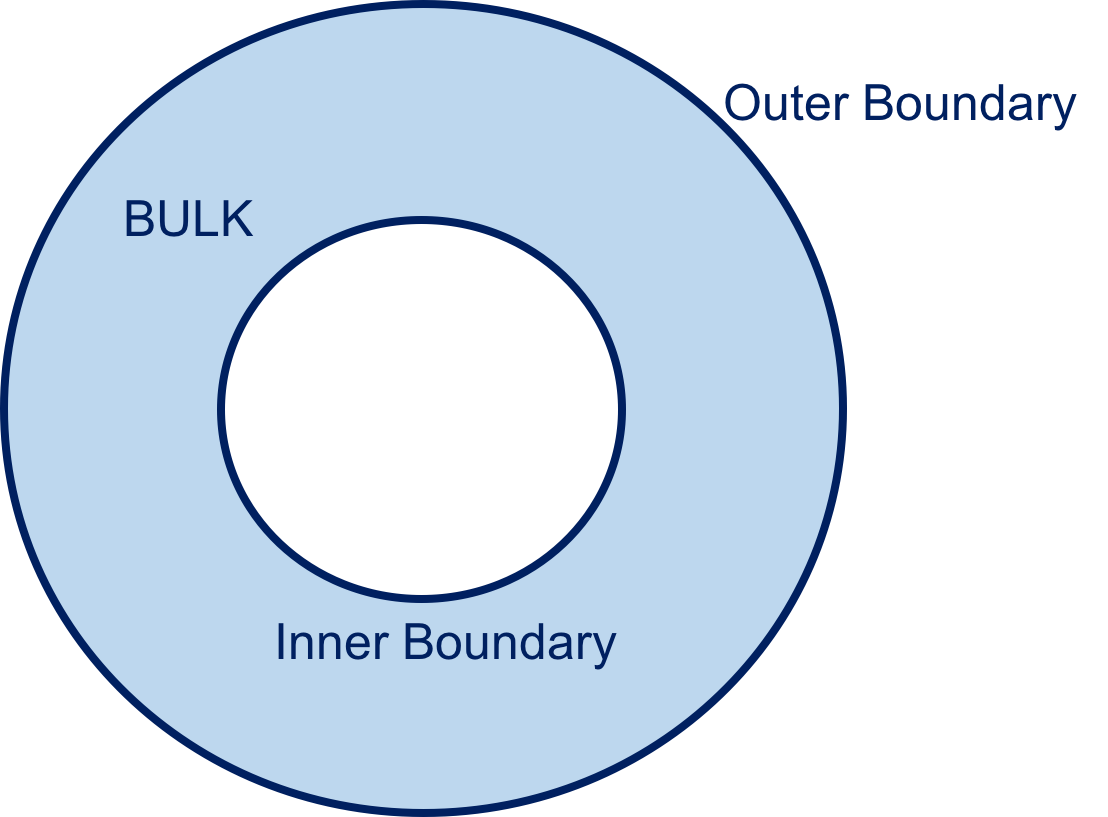
\includegraphics[width=0.4\textwidth]{Smarr}
\end{tabular}
& \begin{tabular}{l}
\parbox{0.5\linewidth}{\begin{itemize}
\setbeamertemplate{itemize items}[triangle]
\setlength{\parskip}{5pt}
\item Outer Boundary $\partial \Sigma^{\text{out}}$
\item Bulk $\Sigma$
\item Inner Boundary $\partial \Sigma^{\text{int}}$
\setbeamertemplate{itemize items}[default]
\end{itemize}}
\end{tabular}  \\
\end{tabular}

\item<2-> Stokes's Theorem:
\begin{align}
\int\limits_{\Sigma} d A_{p} = \int\limits_{\partial \Sigma^{\text{out}}} A_{p} - \int\limits_{\partial \Sigma^{\text{int}}} A_{p} \notag
\end{align}

\end{itemize}
\end{frame}

%------------------------------------------------ 

\begin{frame}
\frametitle{Topology}

\begin{itemize}
\setlength{\parskip}{10pt}
\item Spaces with two boundaries

\vspace{0.5em}

\begin{tabular}{cl}  
\begin{tabular}{c}
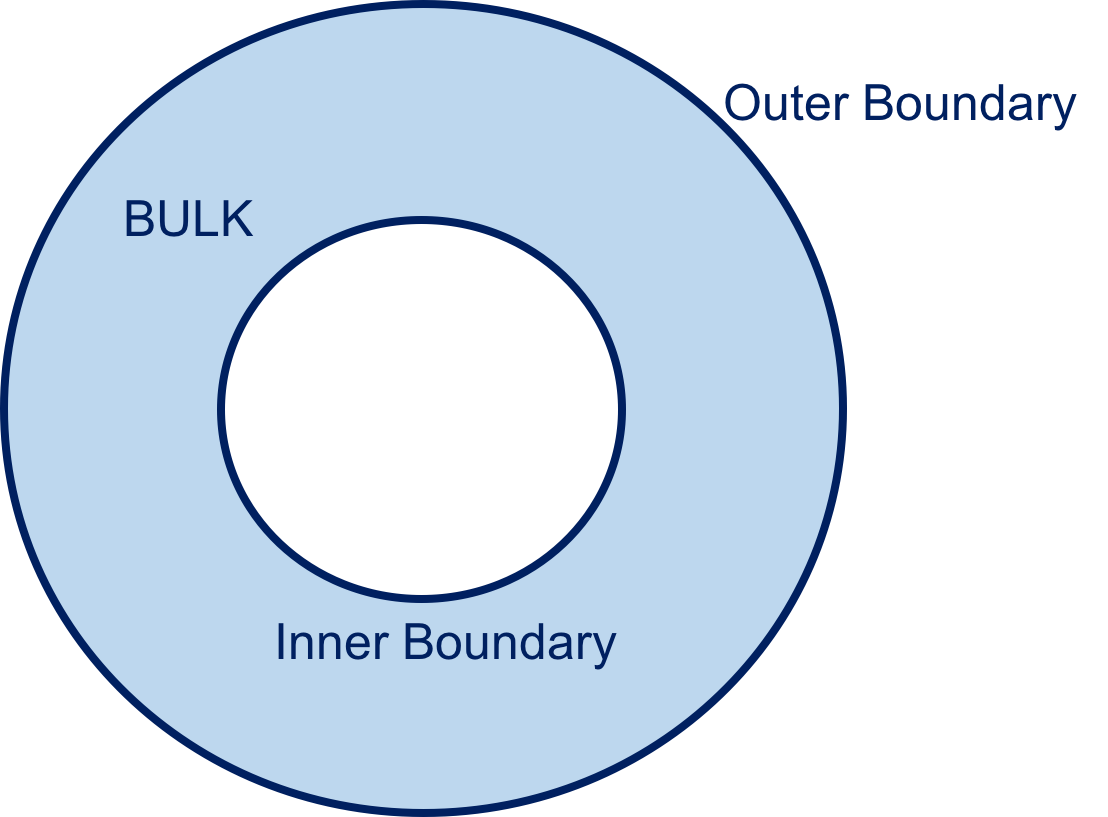
\includegraphics[width=0.4\textwidth]{Smarr}
\end{tabular}
& \begin{tabular}{l}
\parbox{0.5\linewidth}{\begin{itemize}
\setbeamertemplate{itemize items}[triangle]
\setlength{\parskip}{5pt}
\item Outer Boundary $\partial \Sigma^{\text{out}}$
\item Bulk $\Sigma$
\item Inner Boundary $\partial \Sigma^{\text{int}}$
\setbeamertemplate{itemize items}[default]
\end{itemize}}
\end{tabular}  \\
\end{tabular}

\item Stokes's Theorem:
\begin{align}
\int\limits_{\Sigma} d *dK = \int\limits_{\partial \Sigma^{\text{out}}} *dK - \int\limits_{\partial \Sigma^{\text{int}}} *dK \notag
\end{align}

\end{itemize}
\end{frame}

%------------------------------------------------ 

\begin{frame}
\frametitle{Topology}

\begin{itemize}
\setlength{\parskip}{10pt}
\item Spaces with two boundaries

\vspace{0.5em}

\begin{tabular}{cl}  
\begin{tabular}{c}
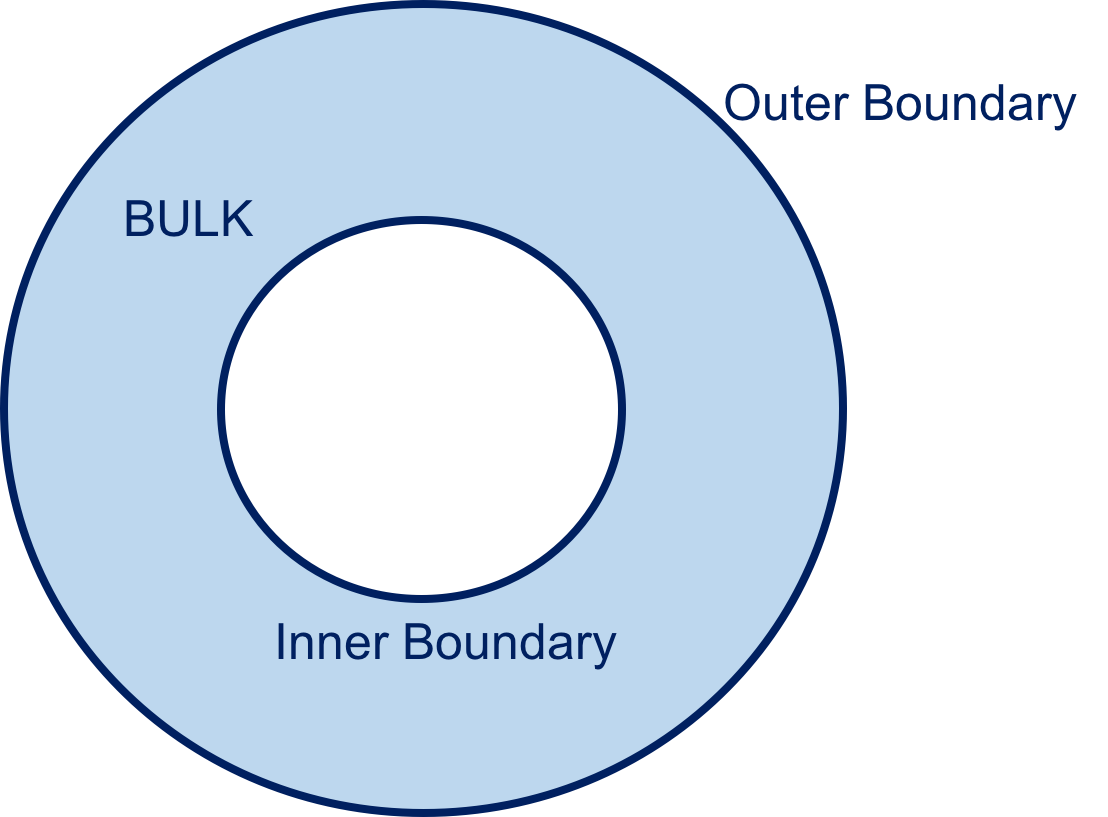
\includegraphics[width=0.4\textwidth]{Smarr}
\end{tabular}
& \begin{tabular}{l}
\parbox{0.5\linewidth}{\begin{itemize}
\setbeamertemplate{itemize items}[triangle]
\setlength{\parskip}{5pt}
\item Outer Boundary $\partial \Sigma^{\text{out}}$
\item Bulk $\Sigma$
\item Inner Boundary $\partial \Sigma^{\text{int}}$
\setbeamertemplate{itemize items}[default]
\end{itemize}}
\end{tabular}  \\
\end{tabular}

\item Stokes's Theorem:
\begin{align}
\int\limits_{\Sigma} d *dK = \underbrace{\int\limits_{\partial \Sigma^{\text{out}}} *dK}_{Q_{K}} - \int\limits_{\partial \Sigma^{\text{int}}} *dK \notag
\end{align}

\end{itemize}
\end{frame}

%------------------------------------------------ 

\begin{frame}
\frametitle{Topology}

\begin{itemize}
\setlength{\parskip}{10pt}
\item Spaces with two boundaries

\vspace{0.5em}

\begin{tabular}{cl}  
\begin{tabular}{c}
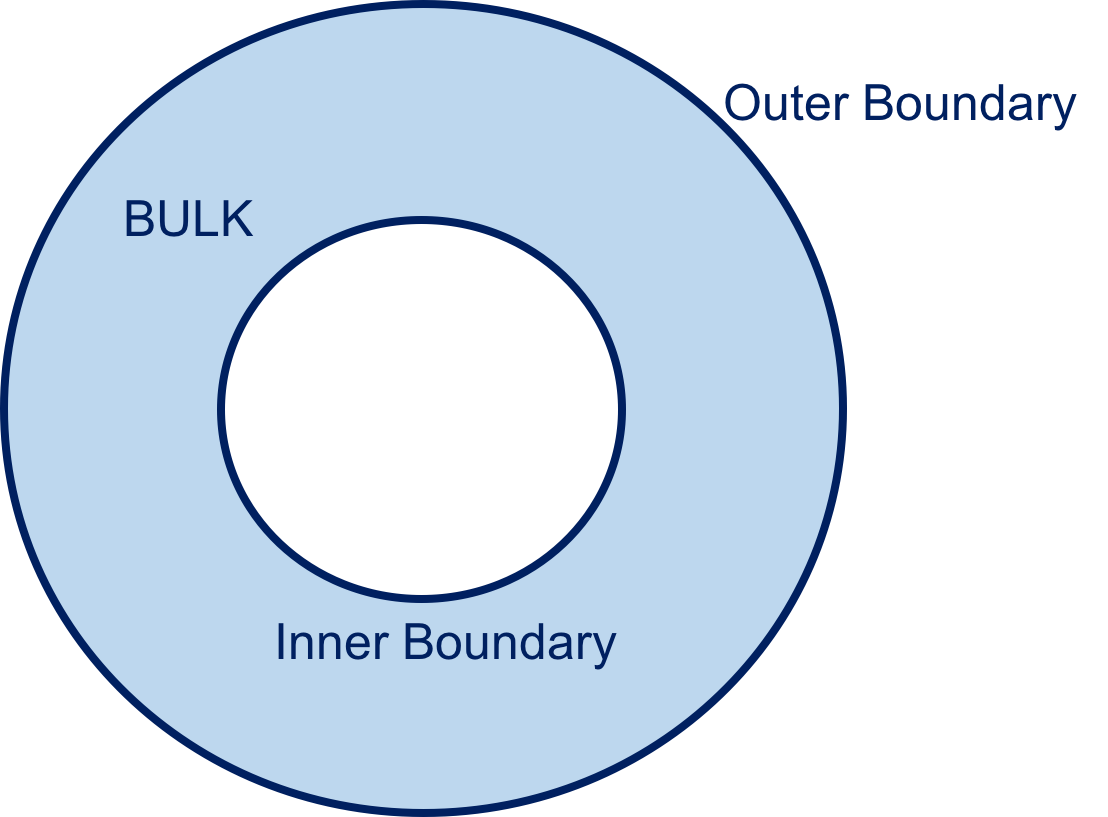
\includegraphics[width=0.4\textwidth]{Smarr}
\end{tabular}
& \begin{tabular}{l}
\parbox{0.5\linewidth}{\begin{itemize}
\setbeamertemplate{itemize items}[triangle]
\setlength{\parskip}{5pt}
\item Outer Boundary $\partial \Sigma^{\text{out}}$
\item Bulk $\Sigma$
\item Inner Boundary $\partial \Sigma^{\text{int}}$
\setbeamertemplate{itemize items}[default]
\end{itemize}}
\end{tabular}  \\
\end{tabular}

\begin{align}
Q_{K} = \int\limits_{\Sigma} d *dK + \int\limits_{\partial \Sigma^{\text{int}}} *dK \notag
\end{align}

\end{itemize}
\end{frame}

%------------------------------------------------ 

\begin{frame}
\frametitle{Topology}

\begin{itemize}
\setlength{\parskip}{10pt}
\item Spaces with two boundaries

\vspace{0.5em}

\begin{tabular}{cl}  
\begin{tabular}{c}
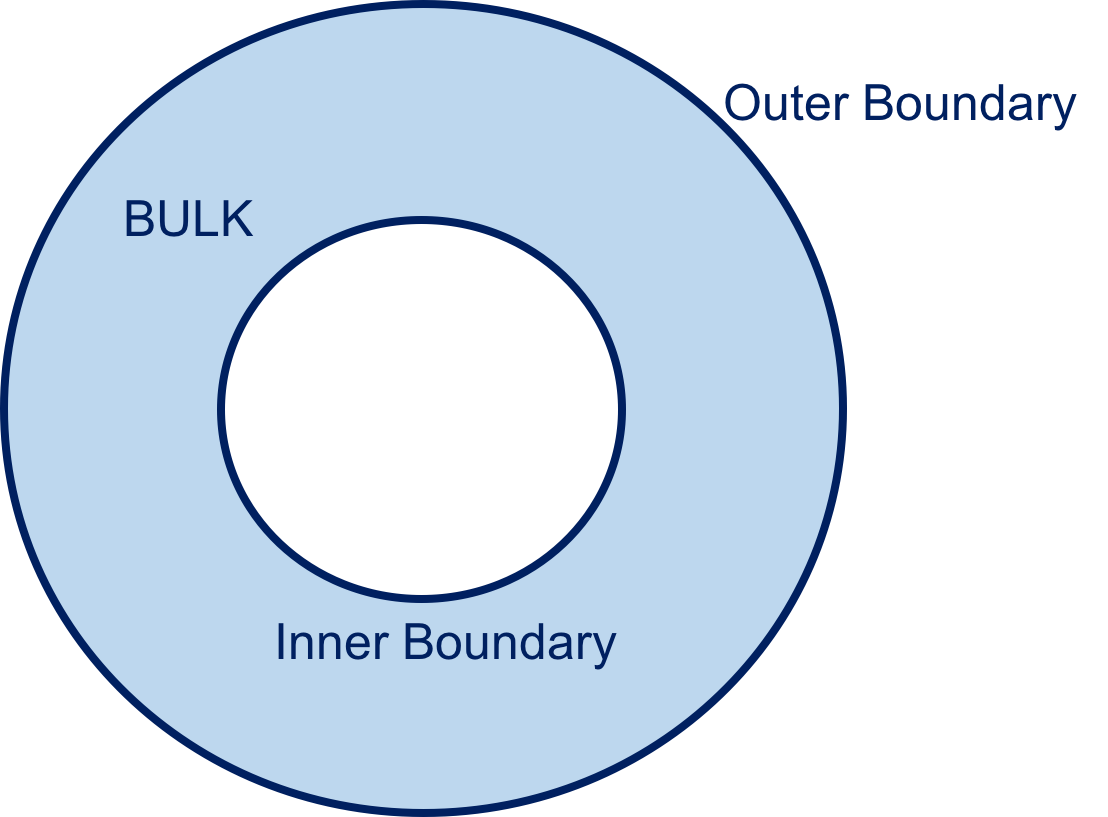
\includegraphics[width=0.4\textwidth]{Smarr}
\end{tabular}
& \begin{tabular}{l}
\parbox{0.5\linewidth}{\begin{itemize}
\setbeamertemplate{itemize items}[triangle]
\setlength{\parskip}{5pt}
\item Outer Boundary $\partial \Sigma^{\text{out}}$
\item Bulk $\Sigma$
\item $\underbrace{\text{Inner Boundary} \:\: \partial \Sigma^{\text{int}}}_{\text{Event Horizon} \:\: \partial \Sigma^{\text{h}}}$
\setbeamertemplate{itemize items}[default]
\end{itemize}}
\end{tabular}  \\
\end{tabular}

\begin{align}
\boxed{Q_{K} = \int\limits_{\Sigma} d *dK + \int\limits_{\partial \Sigma^{\text{h}}} *dK} \:\:\:\:\:\:\:\:\: \text{Smarr Formula} \notag
\end{align}

\end{itemize}
\end{frame}

%------------------------------------------------ 

\begin{frame}
\frametitle{Topology}

\begin{itemize}
\item Smarr Formula
\begin{align}
Q_{K} = \int\limits_{\Sigma} d *dK + \int\limits_{\partial \Sigma^{\text{h}}} *dK \notag
\end{align}
\end{itemize}

\end{frame}

%------------------------------------------------ 

\begin{frame}
\frametitle{Topology}

\begin{itemize}
\setlength{\parskip}{10pt}
\item<1-> Smarr Formula
\begin{align}
Q_{K} = \xcancel{\int\limits_{\Sigma} d *dK} + \int\limits_{\partial \Sigma^{\text{h}}} *dK \notag
\end{align}

\item<2-> $Q_K \rightarrow$ Mass (or Energy $dE$)

\item<3-> $\int\limits_{\partial \Sigma^{\text{h}}} *dK  \rightarrow$ Area $dA$ \:\:\:\:\: (Most general case: $dA, dQ, dJ)$

\item<4-> First Law of Black Hole Thermodynamics
\vspace{0.5em}
\begin{align}
dE \sim dA + dQ + dJ \notag
\end{align}
\end{itemize}

\end{frame}
%------------------------------------------------ 

\begin{frame}
\frametitle{Topology}

\begin{itemize}
\setlength{\parskip}{10pt}
\item Smarr Formula
\begin{align}
Q_{K} =\int\limits_{\Sigma} d *dK +  \xcancel{\int\limits_{\partial \Sigma^{\text{h}}} *dK} \notag
\end{align}

\item $Q_K \rightarrow$ Mass (or Energy $dE$)

\item $\int\limits_{\partial \Sigma^{\text{h}}} *dK  \rightarrow$ Area $dA$ \:\:\:\:\: (Most general case: $dA, dQ, dJ)$

\item First Law of Black Hole Thermodynamics
\vspace{0.5em}
\begin{align}
dE \sim dA + dQ + dJ \notag
\end{align}
\end{itemize}

\end{frame}
%------------------------------------------------ 

\begin{frame}
\frametitle{Topology}
\begin{itemize}
\setlength{\parskip}{10pt}
\item Smarr Formula
\begin{align}
\underbrace{Q_{K}}_{\text{No Divergence}} =\int\limits_{\Sigma} R^{\mu\nu} K_\nu d\Sigma_{\mu} + \int\limits_{\partial \Sigma^{\text{h}}} \nabla^{\mu} K^{\nu} d\Sigma_{\mu\nu} \notag
\end{align}
\end{itemize}
\end{frame}

%------------------------------------------------ 

\begin{frame}
\frametitle{Topology}
\begin{itemize}
\setlength{\parskip}{10pt}
\item Smarr Formula
\begin{align}
\underbrace{Q_{K}}_{\text{No Divergence}} = \underbrace{\int\limits_{\Sigma} R^{\mu\nu} K_\nu d\Sigma_{\mu} + \int\limits_{\partial \Sigma^{\text{h}}} \nabla^{\mu} K^{\nu} d\Sigma_{\mu\nu}}_{\text{We expect no divergence}} \notag
\end{align}
\end{itemize}

\end{frame}
%------------------------------------------------ 

\begin{frame}
\frametitle{Topology}
\begin{itemize}
\setlength{\parskip}{10pt}
\item Smarr Formula
\begin{align}
\underbrace{Q_{K}}_{\text{No Divergence}} = \underbrace{\int\limits_{\Sigma} R^{\mu\nu} K_\nu d\Sigma_{\mu} + \int\limits_{\partial \Sigma^{\text{h}}} \nabla^{\mu} K^{\nu} d\Sigma_{\mu\nu}}_{\text{We expect no divergence}} \notag
\end{align}

\item Adding Killing Potential
\begin{align}
Q_{K} = \int\limits_{\Sigma} \Big( R^{\mu\nu} K_\nu + \Lambda \nabla_\nu \omega^{\mu\nu} \Big) d\Sigma_{\mu} + \int\limits_{\partial \Sigma^{\text{h}}} \Big( \nabla^{\mu} K^{\nu} + \Lambda \omega^{\mu\nu} \Big) d\Sigma_{\mu\nu} \notag
\end{align}
\end{itemize}

\end{frame}
%------------------------------------------------ 
\begin{frame}
\frametitle{Topology}
\begin{itemize}
\setlength{\parskip}{8pt}
\item Smarr Formula
\begin{align}
\underbrace{Q_{K}}_{\text{No Divergence}} = \underbrace{\int\limits_{\Sigma} R^{\mu\nu} K_\nu d\Sigma_{\mu} + \int\limits_{\partial \Sigma^{\text{h}}} \nabla^{\mu} K^{\nu} d\Sigma_{\mu\nu}}_{\text{We expect no divergence}} \notag
\end{align}

\item Adding Killing Potential
\begin{align}
Q_{K} = \int\limits_{\Sigma} \Big( R^{\mu\nu} K_\nu + \Lambda \underbrace{\nabla_\nu \omega^{\mu\nu}}_{-K^\mu} \Big) d\Sigma_{\mu} + \int\limits_{\partial \Sigma^{\text{h}}} \Big( \nabla^{\mu} K^{\nu} + \Lambda \omega^{\mu\nu} \Big) d\Sigma_{\mu\nu} \notag
\end{align}
\end{itemize}

\end{frame}
%------------------------------------------------ 

\begin{frame}
\frametitle{Topology}
\begin{itemize}
\setlength{\parskip}{8pt}
\item Smarr Formula
\begin{align}
\underbrace{Q_{K}}_{\text{No Divergence}} = \underbrace{\int\limits_{\Sigma} R^{\mu\nu} K_\nu d\Sigma_{\mu} + \int\limits_{\partial \Sigma^{\text{h}}} \nabla^{\mu} K^{\nu} d\Sigma_{\mu\nu}}_{\text{We expect no divergence}} \notag
\end{align}

\item Adding Killing Potential
\begin{align}
Q_{K} = \int\limits_{\Sigma} \Big( R^{\mu\nu} K_\nu + \Lambda \underbrace{\nabla_\nu \omega^{\mu\nu}}_{-K^\mu} \Big) d\Sigma_{\mu} + \int\limits_{\partial \Sigma^{\text{h}}} \Big( \nabla^{\mu} K^{\nu} + \Lambda \omega^{\mu\nu} \Big) d\Sigma_{\mu\nu} \notag
\end{align}

\item Remember: $R_{\mu\nu} = \Lambda g_{\mu\nu}$ $\rightarrow$ $R^{\mu\nu} K_\nu = \Lambda K^\mu $

\end{itemize}

\end{frame}
%------------------------------------------------

\begin{frame}
\frametitle{Topology}
\begin{itemize}
\setlength{\parskip}{8pt}
\item Smarr Formula
\begin{align}
\underbrace{Q_{K}}_{\text{No Divergence}} = \underbrace{\int\limits_{\Sigma} R^{\mu\nu} K_\nu d\Sigma_{\mu} + \int\limits_{\partial \Sigma^{\text{h}}} \nabla^{\mu} K^{\nu} d\Sigma_{\mu\nu}}_{\text{We expect no divergence}} \notag
\end{align}

\item Adding Killing Potential
\begin{align}
Q_{K} = \int\limits_{\Sigma} \Big( R^{\mu\nu} K_\nu + \Lambda \underbrace{\nabla_\nu \omega^{\mu\nu}}_{-K^\mu} \Big) d\Sigma_{\mu} + \int\limits_{\partial \Sigma^{\text{h}}} \Big( \nabla^{\mu} K^{\nu} + \Lambda \omega^{\mu\nu} \Big) d\Sigma_{\mu\nu} \notag
\end{align}

\item Remember: $R_{\mu\nu} = \Lambda g_{\mu\nu}$ $\rightarrow$ $R^{\mu\nu} K_\nu = \Lambda K^\mu $

\item Bulk $\rightarrow$ Free of divergences! $\checkmark$
\end{itemize}

\end{frame}
%------------------------------------------------

\begin{frame}
\frametitle{Summing Up}

\begin{itemize}
\setlength{\parskip}{10pt}

\item Putting everything together

\begin{itemize}
\setbeamertemplate{itemize items}[triangle]
\setlength{\parskip}{5pt}
\item Cosmological Constant $\rightarrow$ Killing Potential
\item Topology $\rightarrow$ Smarr Formula
\item Inner Boundary = Event Horizon
\item No divergence at infinity and in the bulk!
\setbeamertemplate{itemize items}[default]
\end{itemize}

\vspace{0.5em}
\begin{align}
\boxed{
M = \int\limits_{\Sigma} R^{\mu\nu} K_\nu d\Sigma_{\mu} + \int\limits_{\partial\Sigma^{\text{h}}} \Big( \nabla^\mu K^{\nu} + \Lambda \omega^{\mu\nu} \Big) d\Sigma_{\mu\nu}} \notag
\end{align}

\end{itemize}
\end{frame}

%------------------------------------------------ 

\begin{frame}
\frametitle{Overview}

\begin{itemize}
\setlength{\parskip}{10pt}
\item Include Cosmological Constant $\Lambda$ (AdS Spacetime) $\checkmark$
\item Include Topology $\checkmark$
\item \boxed{\text{Include Matter Fields (Non - Empty Spacetime)}}
\item Interpret the result. Why 4 dimensions are not enough!
\item Moving to String Theory
\end{itemize}
\end{frame}

%------------------------------------------------ 

\begin{frame}
\frametitle{Matter Fields}

\begin{itemize}
\setlength{\parskip}{10pt}

\item<1-> Non-Empty Spacetime $\rightarrow$ Contribution of the bulk to the mass!

\item<2-> We include Matter Fields
\begin{itemize}
\setbeamertemplate{itemize items}[triangle]
\setlength{\parskip}{5pt}
\item A set of scalar fields $X^I$.
\item A set of $U(1)$ gauge fields $A^I$.
\setbeamertemplate{itemize items}[default]
\setlength{\parskip}{10pt}
\end{itemize}

\item<3-> The Action
\vspace{0.9em}
{\small
\begin{align}
S = \int d^4x \sqrt{-g} \Big( R &- \frac{1}{2} Q_{IJ} \partial_\mu X^I \partial^\mu X^J - \frac{1}{4} Q_{IJ} F^I_{\mu\nu}  F^{J \mu\nu} \Big) - \int C_{IJ} F^I \wedge F^J \notag
\end{align}}

\end{itemize}
\end{frame}


%------------------------------------------------ 

\begin{frame}
\frametitle{Matter Fields}

\begin{itemize}
\setlength{\parskip}{10pt}

\item Non-Empty Spacetime $\rightarrow$ Contribution of the bulk to the mass!

\item We include Matter Fields
\begin{itemize}
\setbeamertemplate{itemize items}[triangle]
\setlength{\parskip}{5pt}
\item A set of scalar fields $X^I$.
\item A set of $U(1)$ gauge fields $A^I$.
\setbeamertemplate{itemize items}[default]
\setlength{\parskip}{10pt}
\end{itemize}

\item The Action
\vspace{0.9em}
{\small
\begin{align}
S = \int d^4x \sqrt{-g} \Big( R &- \frac{1}{2} Q_{IJ} \partial_\mu X^I \partial^\mu X^J - \frac{1}{4} Q_{IJ} F^I_{\mu\nu}  F^{J \mu\nu} \Big) - \underbrace{\int C_{IJ} F^I \wedge F^J}_{\text{Chern-Simons Term}} \notag
\end{align}}

\item Chern-Simons Term: Purely Topological $\rightarrow$ Topological Current

\end{itemize}
\end{frame}


%------------------------------------------------ 

\begin{frame}
\frametitle{Matter Fields}

\begin{itemize}
\setlength{\parskip}{10pt}

\item<1-> Remember
\begin{align}
M = \int\limits_{\Sigma} R^{\mu\nu} K_\nu d\Sigma_{\mu} + \int\limits_{\partial\Sigma^{\text{h}}} \Big( \nabla^\mu K^{\nu} + \Lambda \omega^{\mu\nu} \Big) d\Sigma_{\mu\nu} \notag
\end{align}

\item<2-> We introduce dual field: $G_I = Q_{IJ} * F^J$

\item<3-> Einstein Equations
\begin{align}
R_{\mu\nu} = \frac{1}{2} Q_{IJ} \partial_{\mu} X^I \partial_{\nu} X^J + \frac{1}{4} Q_{IJ} F^I_{\mu\rho} F^{J\rho}_\nu + \frac{1}{4} Q^{IJ} G_{I\mu\rho} G^\rho_{J\nu} \notag
\end{align}

\item<4-> $R^{\mu\nu} K_\nu$ $\rightarrow$  We need to calculate: $K^\mu \partial_\mu X$, $K^\mu F_{\mu\nu}$ and $K^\mu G_{\mu\nu}$

\end{itemize}
\end{frame}


%------------------------------------------------ 

\begin{frame}
\frametitle{Matter Fields}

\begin{itemize}
\setlength{\parskip}{10pt}

\item<1-> \boxed{\text{\textbf{Assumption: Matter Fields respect the isometries.}}}

\item<2-> If $\mathcal{L}_{K} g_{\mu\nu} = 0$, then:
\begin{align}
\mathcal{L}_{K} X^I = 0 \qquad \mathcal{L}_{K} F^I  = 0 \qquad \mathcal{L}_{K} G_I = 0 \notag
\end{align}

\item<3-> $\mathcal{L}_{K} X^I = 0$ $\rightarrow$ $\boxed{K^\mu \partial_\mu X = 0}$ \:\:\: No contribution from scalar fields!

\item<4-> $\mathcal{L}_{K} F^I  = 0$ $\rightarrow$ $d(i_{K} F^I) = 0$ $\implies$ $\boxed{i_{K} F^I = \Lambda^I + d\lambda^I}$

\item<5-> $\mathcal{L}_{K} G_I = 0$ $\rightarrow$ $\boxed{i_{K} G_I = -2C_{IJ} \Lambda^J - 2C_{IJ} d\lambda^J + H_{I} + dh_{I}}$

\item<6-> Important: $\Lambda^I$ and $H^I$ are closed but not exact!
\end{itemize}
\end{frame}

%------------------------------------------------ 

\begin{frame}
\frametitle{Matter Fields}

\begin{itemize}
\setlength{\parskip}{10pt}

\item<1-> Substituting to Smarr Formula
\vspace{0.8em}
\begin{align}
M = \int\limits_{\Sigma} \Lambda^I \wedge (G_I + 2C_{IJ} \wedge F^J ) +  H_{I} \wedge F^I
+ \int\limits_{\partial\Sigma^{\text{h}}}\text{``something''} \notag
\end{align}

\item<2-> ``something'': $\nabla K$, $\Lambda \omega$, $\lambda^I$ and $h_I$

\item<3-> Finally, we can remove the event horizon!
\vspace{0.8em}
\begin{align}
\boxed{
M  = \frac{1}{32\pi G_{4}} \int\limits_{\Sigma} \Lambda^I \wedge (G_I + 2C_{IJ} \wedge F^J ) +  H_{I} \wedge F^I}\notag
\end{align}


\end{itemize}
\end{frame}

%-------------------------------------

\begin{frame}
\frametitle{Overview}

\begin{itemize}
\setlength{\parskip}{10pt}
\item Include Cosmological Constant $\Lambda$ (AdS Spacetime) $\checkmark$
\item Include Topology $\checkmark$
\item Include Matter Fields (Non - Empty Spacetime) $\checkmark$
\item \boxed{\text{Interpret the result. Why 4 dimensions are not enough!}}
\item Moving to String Theory
\end{itemize}
\end{frame}

%------------------------------------------------ 

\begin{frame}
\frametitle{Interpreting the result}

\begin{align}
M =& \frac{1}{32\pi G_{4}} \int\limits_{\Sigma} \Big( \Lambda^I \wedge (G_I + 2C_{IJ} \wedge F^J ) + H^I \wedge F_{I}   \Big)\notag
\end{align}

\begin{itemize}
\setlength{\parskip}{10pt}

\item<2-> $H^p(M) = \frac{\text{Group of Closed p-Forms}}{\text{Group of Exact p-Forms}}$

\item<3-> Cohomology $H^r(M)$ says which forms are allowed by the topology!

\item<4-> e.g: Trivial Cohomology $H^{1}(M)= 0$ 

\item<5-> Simply Connected Topological Space $\rightarrow$ $H^{1}(M)= 0$ $\rightarrow$ $M=0$

\item<6-> Adding extra dimensions...
\end{itemize}
\end{frame}

%------------------------------------------------ 

\begin{frame}
\frametitle{Previous Papers}

\begin{itemize}
\setlength{\parskip}{18pt}
\item<1-> 4-D: Just seen!
\item<2-> 5-D: (2014) Global Structure of Five-dimensional BPS Fuzzballs - Gibbons \& Warner (arXiv:1305.0957v1)
\item<3-> 6-D: (2015) Structure of Six-Dimensional Microstate Geometries - Lange, Mayerson \& Vercnocke (arXiv:1504.07987v1)
\item<4-> 11-D: (2014) Smarr's Formula in Eleven-Dimensional Supergravity - Haas (arXiv:1405.3708v1)

\end{itemize}
\end{frame}

%------------------------------------------------ 

\begin{frame}
\frametitle{Previous Papers}

\begin{itemize}
\setlength{\parskip}{18pt}
\item 4-D: Just seen!
\item 5-D: (2014) Global Structure of Five-dimensional BPS Fuzzballs - Gibbons \& Warner (arXiv:1305.0957v1)
\item 6-D: (2015) Structure of Six-Dimensional Microstate Geometries - Lange, Mayerson \& Vercnocke (arXiv:1504.07987v1)
\item \boxed{\text{10-D: Current Project - Supersting Theory}}
\item 11-D: (2014) Smarr's Formula in Eleven-Dimensional Supergravity - Haas (arXiv:1405.3708v1)

\end{itemize}
\end{frame}

%------------------------------------------------ 

\begin{frame}
\frametitle{Overview}

\begin{itemize}
\setlength{\parskip}{10pt}
\item Include Cosmological Constant $\Lambda$ (AdS Spacetime) $\checkmark$
\item Include Topology $\checkmark$
\item Include Matter Fields (Non - Empty Spacetime) $\checkmark$
\item Interpret the result. Why 4 dimensions are not enough! $\checkmark$
\item  \boxed{\text{Moving to String Theory}}
\end{itemize}
\end{frame}

%------------------------------------------------ 


\begin{frame}
\frametitle{Superstring Theory}

\begin{itemize}
\setlength{\parskip}{10pt}
\item<1-> Superstring Theory requires 10 dimensions.

\item<2-> Different types of Superstring Theories.
\begin{figure}[htb]
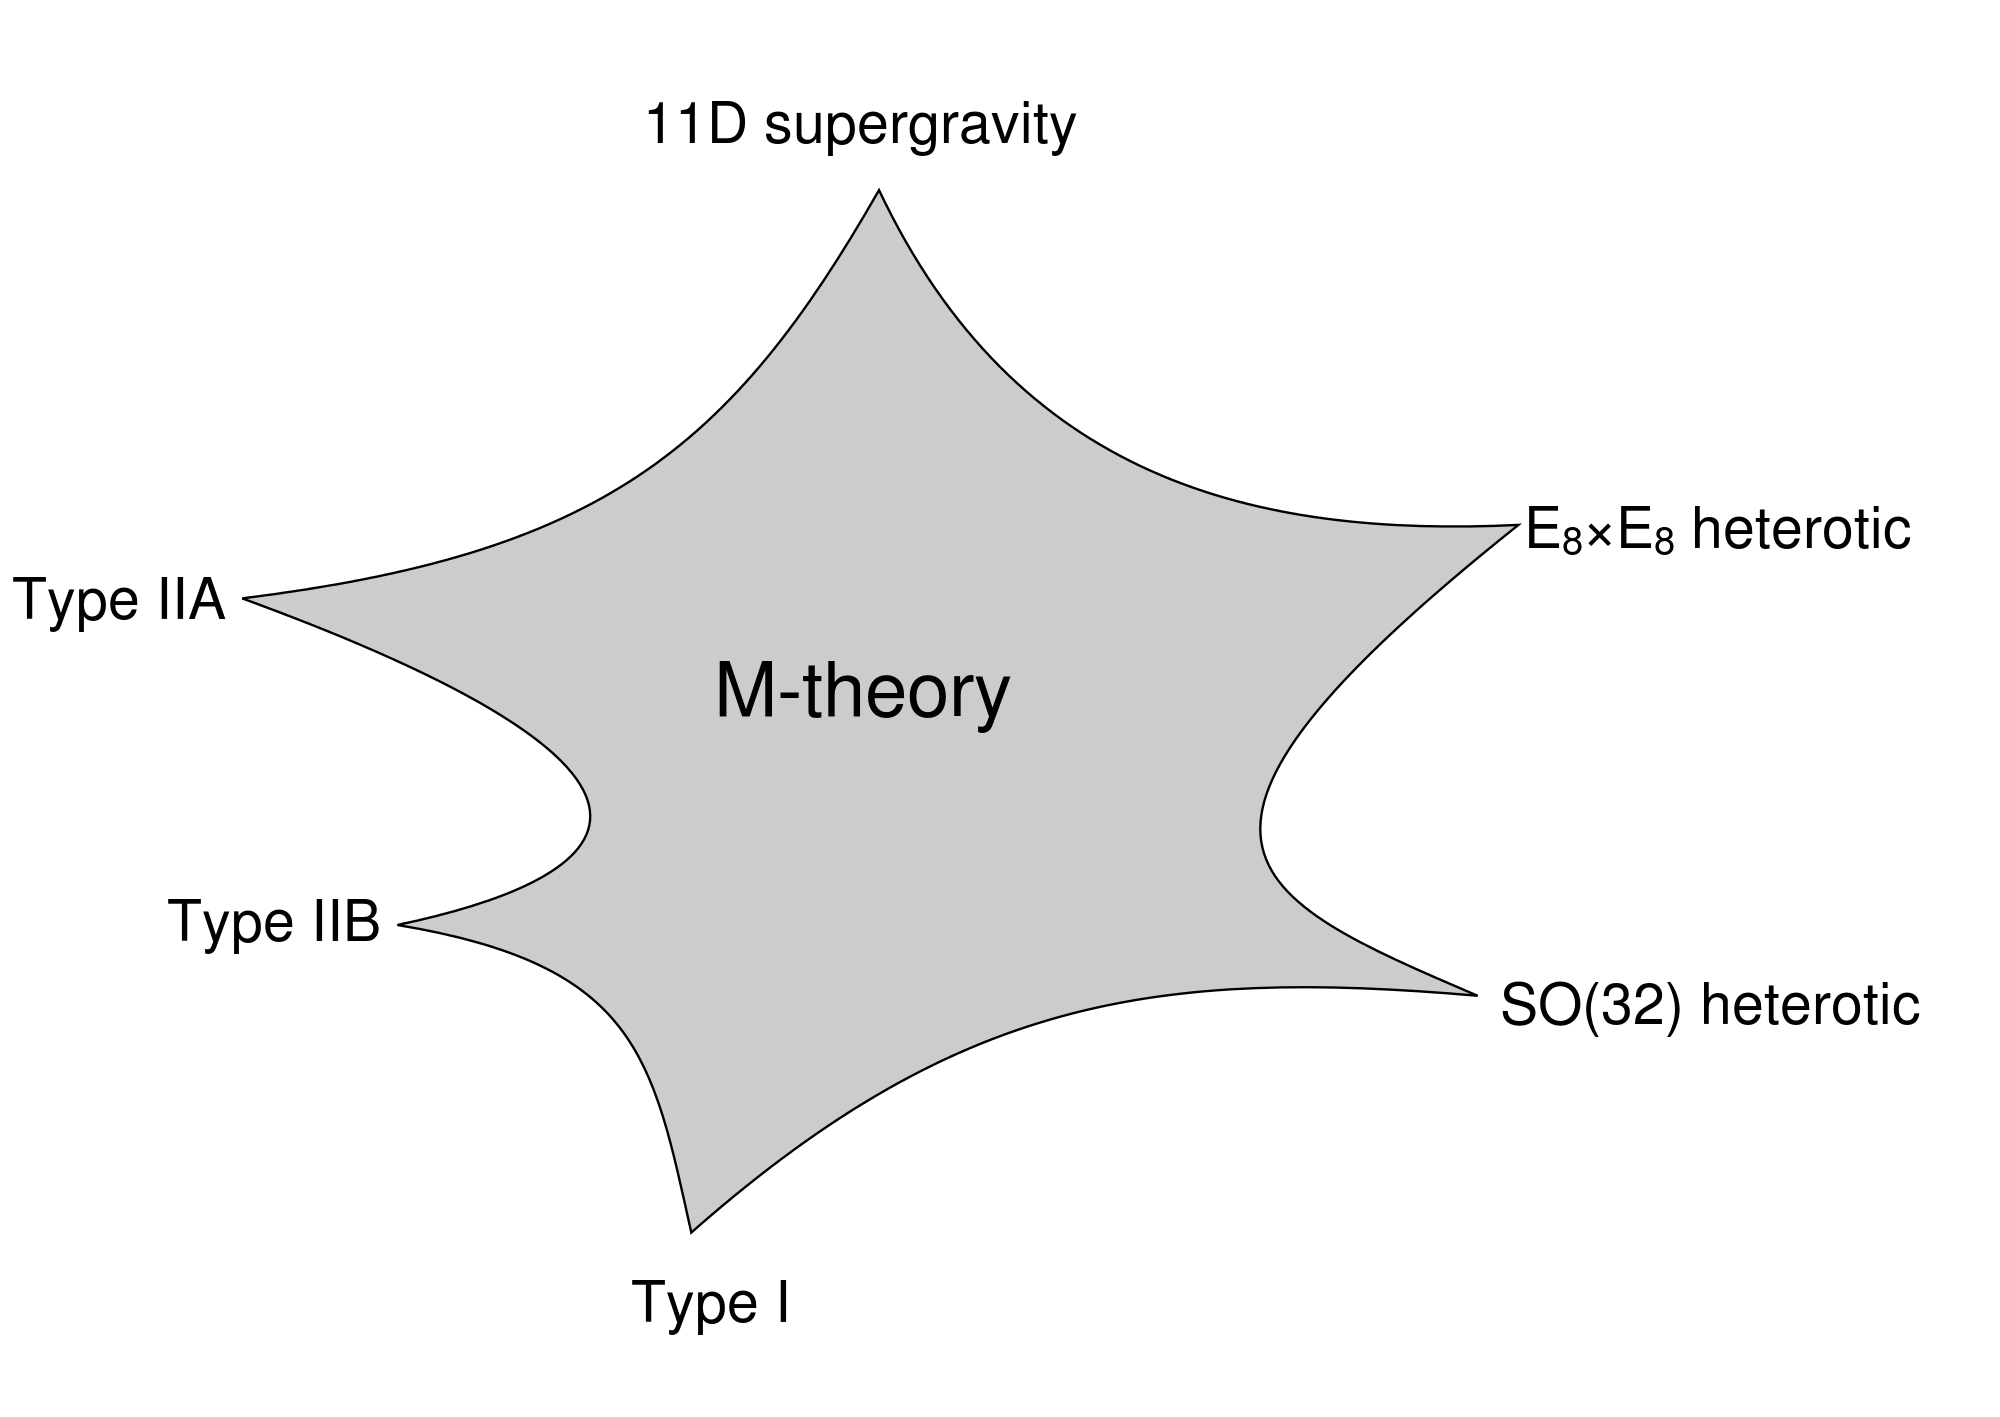
\includegraphics[width=0.45\textwidth]{Mtheory}
\end{figure}

\item<3-> \textbf{Current Project:} IIA Superstring Theory $\xrightarrow[\text{Limit}]{\text{Low Energy}}$ IIA 10-D SUGRA

\end{itemize}
\end{frame}

%------------------------------------------------ 

\begin{frame}
\frametitle{Type II Superstring Theory}

\begin{itemize}
\setlength{\parskip}{10pt}
\item<1-> Fields in Type II Superstring Theory

\begin{itemize}
\setbeamertemplate{itemize items}[triangle]
\setlength{\parskip}{5pt}

\item<2-> \underline{\textbf{NS-NS Sector}}\\
\vspace{10 pt}
Low Energy Limit $\rightarrow$ Massless Fields
\vspace{10 pt}
$$ \alpha^{-1}_\mu \alpha^{-1}_\nu \Ket{0}
\begin{cases}
\text{Symmetric part without Trace} \rightarrow \text{Graviton } g_{\mu\nu}  \\
\text{Antisymmetric part} \rightarrow \text{Antisymmetric 2-form  } B_{\mu\nu} \\
\text{Trace} \rightarrow \text{Dilaton  } \phi
\end{cases}
$$

\item<3-> \underline{\textbf{R-R Sector}}\\
\vspace{10 pt}
Generalisation of gauge fields: $C_p$ with Field Strengths $F_{p} = dC_{p-1}$\\
\footnotesize{($p=0,1, \ldots 10$)}
\setbeamertemplate{itemize items}[default]
\end{itemize}

\item<4-> \textbf{Type IIA}: \:\:\:\:\:\: NS-NS: $g_{\mu\nu}$, $B_2$, $\phi$ \:\:\:\:\:\: R-R: $C_1$, $C_3$, ($C_5$), ($C_7$)

\end{itemize}
\end{frame}

%------------------------------------------------ 

\begin{frame}
\frametitle{Type IIA Superstring Theory}

\begin{itemize}
\setlength{\parskip}{10pt}
\item<1-> Constructing an action: $S_{IIA} = S_\text{NS} + S_{\text{RR}} + S_{\text{CS}}$

\begin{itemize}
\setbeamertemplate{itemize items}[triangle]
\setlength{\parskip}{6pt}
\item<2-> $S_{NS} = \frac{1}{2\kappa^{2}} \int d^{10}x \sqrt{-g} \Big(R - \frac{1}{2} \partial_{\mu} \phi \partial^{\mu} \phi - \frac{1}{2} e^{-\phi} {|H_{3}|}^2 \Big)$
\vspace{6pt}
\item<2-> $S_{RR} = \frac{1}{2\kappa^{2}} \int d^{10}x \sqrt{-g} \Big( - \frac{1}{2} e^{\frac{3\phi}{2}} {|\tilde{F}_{2}|}^2 - \frac{1}{2} e^{\frac{\phi}{2}} {|\tilde{F}_{4}|}^2 \Big)$
\vspace{6pt}
\item<2-> $S_{CS} = - \frac{1}{4\kappa^{2}} \int B_{2} \wedge {\tilde{F}}_{4} \wedge {\tilde{F}}_{4}$
\setbeamertemplate{itemize items}[default]
\end{itemize}

\vspace{5pt}

\item<3-> Fast Forward: Repeat Process of 4 Dimensions $\checkmark$

\begin{itemize}
\setbeamertemplate{itemize items}[triangle]
\setlength{\parskip}{5pt}
\item \small{Einstein Equation - Bianchi Identities - Equations of motion}
\item \small{Define the dual fields and rewrite everything in terms of them}
\item \small{$\mathcal{L}_{K} \text{(all fields)} = 0$ $\rightarrow$ Solve the equations}
\item \small{Substitute everything into Smarr Formula}
\setbeamertemplate{itemize items}[default]
\end{itemize}
\end{itemize}
\end{frame}

%------------------------------------------------

\begin{frame}
\frametitle{Type IIA Superstring Theory}

{\small
\begin{align}
M = &\int\limits_{\Sigma} \Lambda_2 \wedge f(\text{fields}) + \Lambda_6 \wedge H^{*}_3 + \sum_{n}^{1,3,5,7} \Omega_n \wedge \Big( \tilde{F}^{*}_{9-n} + C^{*}_{6-n} \wedge H^{*}_3  \Big) \wedge e^{B_2} \notag
\end{align}}

\begin{itemize}
\setlength{\parskip}{10pt}

\item<2-> $\Lambda_2$ comes from $H_3$. Assumption: $H^2(M) \not= 0$
\item<2-> $\Lambda_6$ comes from $H_7$. Assumption: $H^6(M) \not= 0$
\item<2-> All $\Omega_n$ come from RR sector. Assumption: $H^{2n+1}(M) \not= 0$
\item<3-> More Harmonic Forms give us more freedom on choosing the topology!
\item<4-> More dimensions can easily produce a non-zero mass!

\end{itemize}


\end{frame}

%------------------------------------------------

\begin{frame}
\frametitle{Summary}

\begin{itemize}
\setlength{\parskip}{10pt}
\item<1-> Komar Integral: A way to measure conserved quantities!

\begin{itemize}
\setbeamertemplate{itemize items}[triangle]
\setlength{\parskip}{5pt}
\item Modify in case of AdS spacetime. (Among solutions: Killing Potential)
\item Expand in order to include topology (Smarr Formula)
\setbeamertemplate{itemize items}[default]
\end{itemize}

\item<2->  Add Matter Fields $\rightarrow$ Contribution of the bulk to the conserved charge!

\item<3->  Cohomology shows that 4-d case is not that interesting!

\item<4->  Type IIA Supersting Theory in $d=10$

\item<5->  Extra dimensions give us more freedom on choosing topological spaces!

\end{itemize}
\end{frame}

%------------------------------------------------ 

\begin{frame}
\frametitle{Outlook}

\begin{itemize}
\setlength{\parskip}{10pt}

\item<1->  Behaviour of the solutions to the problem of AdS Komar Integral in the bulk (e.g: G,H Formalism)

\item<2->  Repeat procedure for Type IIB Superstring Theory (Even Harmonic Forms)

\item<3->  Compactification of 10-d result $\rightarrow$ Obtain the 4-d, 5-d and 6-d results (Previous papers)

\item<4-> Apply specific geometries and calculate explicitly the mass!

\begin{itemize}
\setbeamertemplate{itemize items}[triangle]
\setlength{\parskip}{5pt}
\item e.g: Lin, Lunin, Maldacena Geometries $(AdS_5 \times S_5)$
\item e.g: Any geometry of the form $(AdS_p \times S_q)$
\item Expectation: $M \sim \sum_{n} Q_{n}$, where $Q_{n}$ are the brane's charges
\setbeamertemplate{itemize items}[default]
\end{itemize}
\end{itemize}
\end{frame}

%------------------------------------------------ 

\begin{frame}[c]
\frametitle{The End}

\begin{center}
\Huge Thanks for your attention!
\end{center}

\end{frame}
\end{document} 